\textbf{Pregunta 6}
Decimos que un árbol binario de búsqueda $T_1$ puede ser \textsc{right-converted} a un árbol binario
de búsqueda $T_2$ si es posible obtener $T_2$ de $T_1$ por a tráves de una serie de llamadas a la operación
\textsc{right-rotate}.
\begin{itemize}
\item Da un ejemplo de dos árboles $T_1$ y $T_2$ tal que  $T_1$ no pueda ser \textsc{right-converted} en $T_2$.

\begin{center}
  \begin{figure}[h]
    \centering
    \subfloat[T1]{
      \label{f:T1}
      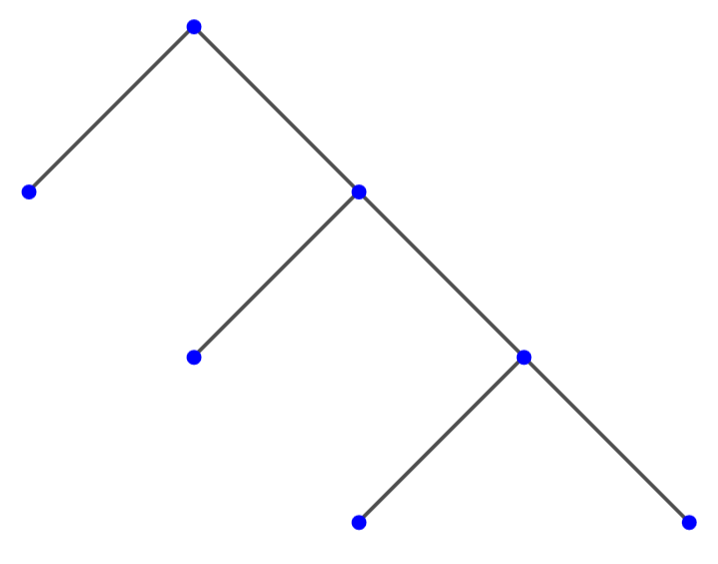
\includegraphics[width=0.4\textwidth]{T1.png}}
    \subfloat[T2]{
      \label{f:T2}
      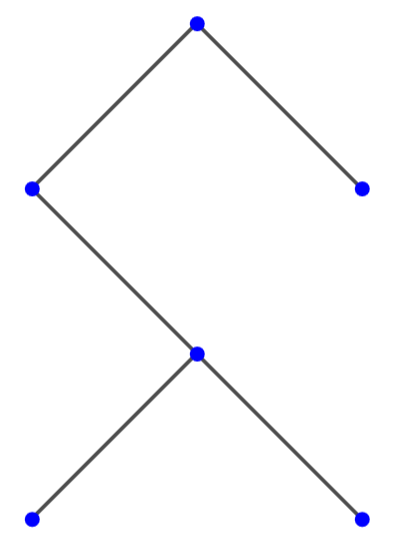
\includegraphics[width=0.25\textwidth]{T2.png}}
    \caption*{Árboles no reducibles por rotación.}
    \label{f:animales}
  \end{figure}


  %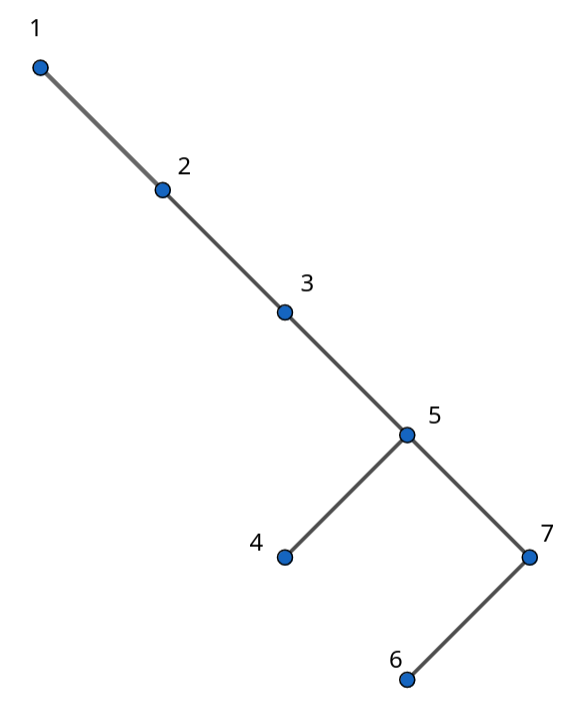
\includegraphics[scale=0.3]{./02.png}
\end{center}


\item Demuestra que si un árbol $T_1$ puede ser \textsc{right-converted} a $T_2$, entonces $T_1$ puede ser
  \textsc{right-converted} usando $O(n^2)$ operaciones \textsc{right-rotate}.\newline

Observemos el peor caso para transformar $T_1$ a $T_2$ por medio de \textsc{right-converted}. Este se da cuándo
$T_2$ es totalmente inverso a $T_1$, esto es, para el vértice raíz rotemos hacia la derecha $n - 1$ veces,
para los nodos hijos rotemos $n - 2$ y $n - 3$ veces de manera respectiva de izquierda a derecha. Si aplicamos
estos pasos de manera iterativa podemos concluir que el número de rotaciones necesarias para transformar $T_1$
en $T_2$ son
\[(n - 1) + (n - 2) + \dotsm + 2 + 1 = \frac{n(n - 1)}{2} \in \mathcal{O}(n^2)\]
por lo que tenemos un orden de rotaciones cuadrático.
\end{itemize} 
